\chapter{Pressure}

Comparisons between measurement and prediction of compartment pressure for the NIST/NRC test series and two of the NBS furniture tests are shown in of Appendix A.  Figure \ref{fig:Pressure_Scatter} shows a comparison of predicted and measured values for compartment pressure, along with a summary of the relative difference for the tests.

\begin{figure}
\begin{center}
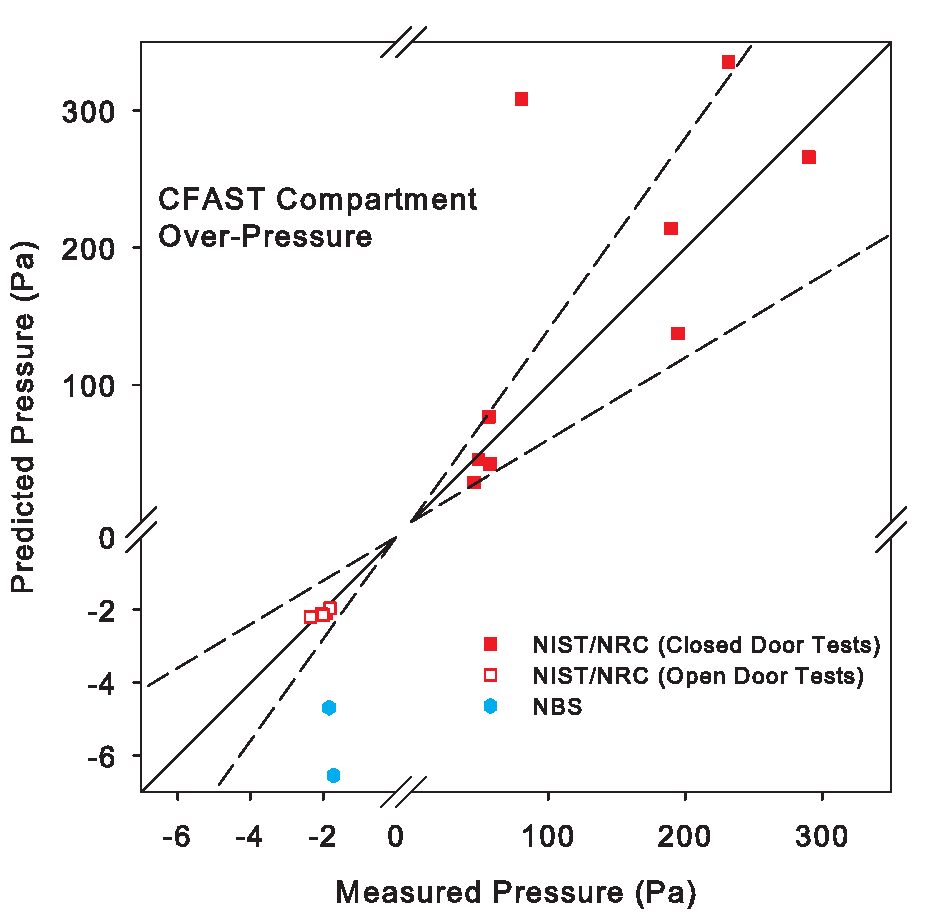
\includegraphics[width=4.0in]{FIGURES/ScatterPlots/Pressure}  \\
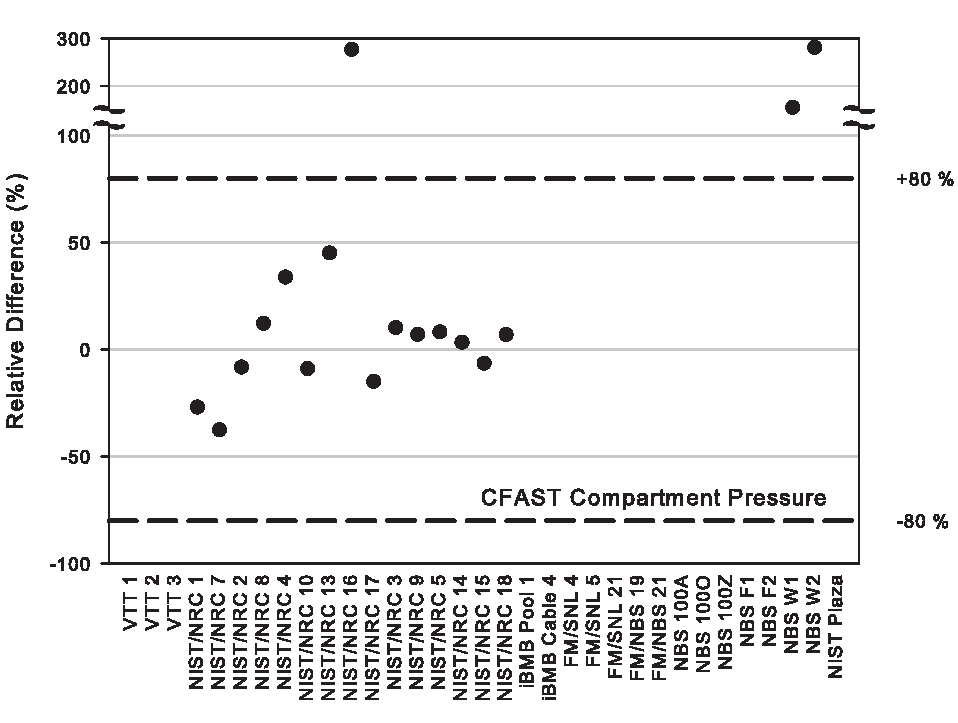
\includegraphics[width=4.0in]{FIGURES/Relative_Diff/Pressure}  
\end{center}
\caption{Comparison of Measured and Predicted Compartment Pressure.} \label{fig:Pressure_Scatter}
\end{figure}

For those tests in which the door to the compartment is open, the magnitude of the pressures are only a few Pascals; however, when the door is closed, the over-pressures are several hundred Pascals.  For both the open- and closed-door tests, CFAST predicts the pressure to within experimental uncertainty with exceptions.  The most notable exception is Test 16, which involved a large (2.3 MW) fire with the door closed and the ventilation on.  By contrast, Test 10 involved a 1.2 MW fire with comparable geometry and ventilation.  There is considerable uncertainty in the magnitude of both the supply and return mass flow rates for Test 16.  Compared to Test 16, Test 10 involves a greater measured supply velocity and a lesser measured exhaust velocity.  This is probably the result of the higher pressure caused by the larger fire in Test 16.  CFAST does not adjust the ventilation rate based on the compartment pressure until a specified cutoff pressure is reached.  This is also the most likely explanation for the over-prediction of compartment pressure in Test 16.

In general, prediction of pressure in CFAST in closed compartments is critically dependent on correct specification of the leakage from the compartment.  Compartments are rarely entirely sealed, and small changes in the leakage area can produce significant changes in the predicted over-pressure.

By comparison, the large relative differences for the two NBS compartment tests with furniture and wall-burning are qualitatively difference than the NIST/NRC outlier.  For these two tests, the difference between model and experiment are on the order of 2 Pa rather than the more than 100 Pa of the NIST/NRC test.  Qualitatively, the comparison between model and experiment for the NBS tests show similar curve shapes but with a notable single spike in the experimental measurements which particularly effects the comparison of peak values.

Based on the model physics and comparisons of model predictions with experimental measurements, CFAST calculations of pressure are seen as appropriate for the tests considered with the following reasons:

\begin{itemize}
\item With exceptions, CFAST predicts compartment pressures within experimental uncertainty.
\item Prediction of compartment pressure for closed-door tests is critically dependent on correct specification of the leakage from the compartment.
\end{itemize}


